% Apêdice
\apendice
\chapter{Questionário} \label{ch:apendice-a}

Este apêndice apresenta a versão em português dos questionários de tipo 1 (\ref{sec:apendice-a-tipo-1}) e 2 (\ref{sec:apendice-a-tipo-2}) aplicados com os participantes do estudo apresentado no capítulo \ref{ch:avaliacao}, intitulado ``Avaliação''. Através desses questionários foram coletados os feedbacks de 16 contribuidores dos projetos Jetty e VRaptor. Todas as questões foram opcionais.

\section{Tipo 1} \label{sec:apendice-a-tipo-1}

\begin{framed}
  \noindent \textit{\textbf{\toolName}}
  \par
  \par
  \noindent \textit{Este questionário é parte de um projeto de pesquisa que propõe uma ferramenta de visualização de software que ajuda os desenvolvedores a gerenciar o desempenho dos sistemas de software, em termos de tempo de execução/resposta. Estamos atualmente conduzindo um estudo sobre o framework \underline{Jetty/VRaptor} e ficaríamos gratos se você pudesse responder as perguntas abaixo.}
  \par
  \noindent \textit{Um conceito importante para o estudo é o cenário. Ele é definido pela interação entre os stakeholders e o sistema. Neste estudo, um cenário foi definido como um caso de teste automatizado do sistema.}
\end{framed}
	
\begin{framed}
	\noindent \textit{\textbf{Página 1/5}}
	\par
	\noindent \textit{\textbf{Questão 1.} Qual sua ocupação atual no seu trabalho?}
	\par
	\noindent \textit{\textbf{Questão 2.} Quantos anos de experiência você possui no desenvolvimento de software em Java?}
	\par
	\noindent \textit{\textbf{Questão 3.} Quantas contribuições você fez para o projeto \underline{Jetty/VRaptor} nos últimos 12 meses?}
\end{framed}

\begin{framed}
	\noindent \textit{\textbf{Página 2/5 - Atributo de Qualidade de Desempenho}}
	\par
	\noindent \textit{\textbf{Questão 4.} Você costuma usar ou já usou alguma ferramenta de análise de desempenho (ferramentas de profiling, APM) no \underline{Jetty/VRaptor}?}
	\par
	\noindent \textit{\textbf{Questão 5.} Se você respondeu ``Uso essas ferramentas frequentemente'' ou ``Já usei essas ferramentas'' na pergunta anterior, você poderia especificar qual(is) ferramenta(s) você usa ou já usou?}
	\par
	\noindent \textit{\textbf{Questão 6.} Suponha que uma funcionalidade do \underline{Jetty/VRaptor} foi evoluída (por você ou outro membro da equipe). O que você faz para garantir que o tempo de execução/resposta de tal funcionalidade é aceitável em comparação com outras releases?}
\end{framed}

\begin{framed}
	\noindent \textit{\textbf{Página 3/5 - Grafo de Chamadas}}
	\par
	\noindent \textit{A figura abaixo mostra uma breve explicação da visualização interativa do Grafo de Chamadas, que mostra os métodos que potencialmente causaram um desvio de desempenho para um determinado cenário (executado através de um caso de teste automatizado) do \underline{Jetty/VRaptor}.}

	\noindent \textit{As próximas perguntas se referirão a uma visualização concreta da evolução de uma release do projeto \underline{Jetty/VRaptor}. Use versões recentes do Google Chrome ou Mozilla Firefox para abrir os links das visualizações da ferramenta.}
	
   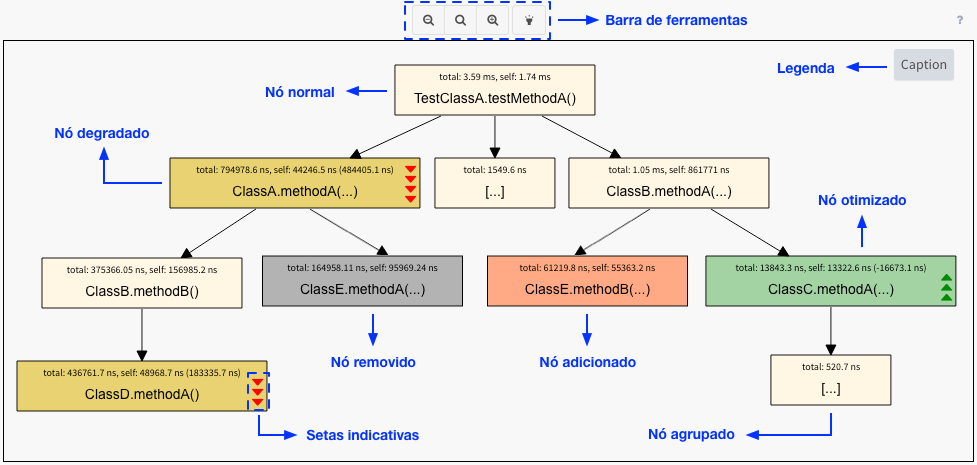
\includegraphics[scale=0.41]{Imagens/call_graph_explicative_portuguese.png}

	\noindent \textit{\textbf{Questão 7.} Considerando a visualização "Grafo de Chamadas" para o caso de teste {\(<\)}nome\_do\_caso\_de\_teste{\(>\)} acessado através do link {\(<\)}link\_para\_a\_ferramenta{\(>\)}, você consegue identificar os possíveis métodos responsáveis pelo desvio de desempenho do cenário? Liste tais métodos em dois grupos: otimizados e degradados.}
	\par
	\noindent \textit{\textbf{Questão 8.} Quão fácil foi responder à pergunta anterior?}
	\par
	\noindent \textit{\textbf{Questão 9.} Considerando a visualização "Grafo de Chamadas" da ferramenta acessada através do link {\(<\)}link\_para\_a\_ferramenta{\(>\)}, identifique o hash do commit responsável pelo principal desvio de desempenho do sistema.}
	\par
	\noindent \textit{\textbf{Questão 10.} Quão fácil foi responder à pergunta anterior?}
	\par
	\noindent \textit{\textbf{Questão 11.} Este desvio parece plausível de acordo com o seu conhecimento do sistema?}
	\par
	\noindent \textit{\textbf{Questão 12.} Você poderia mencionar aspectos dessa visualização que você gostou? E quais outros aspectos você não gostou? Você tem alguma sugestão de melhoria ou comentário para essa visualização?}
\end{framed}

\begin{framed}
	\noindent \textit{\textbf{Página 4/5 - Sumarização de Cenários}}
	\par
	\noindent \textit{O link abaixo fornece os dados brutos para os cenários (executados através de um caso de teste automatizado) com desvios de desempenho para duas versões do \underline{Jetty/VRaptor}: {\(<\)}link\_para\_a\_ferramenta{\(>\)}.}
	\par
	\noindent \textit{\textbf{Questão 13.} Considerando os dados acessados através do link acima, você consegue identificar qual cenário (isto é, caso de teste) possui maior desvio de desempenho (degradação ou melhoria do tempo de execução/tempo de resposta) dentre os exibidos? O cenário foi otimizado ou degradado?}
	\par
	\noindent \textit{\textbf{Questão 14.} Quão fácil foi responder à pergunta anterior?}
	\par
	\noindent \textit{\textbf{Questão 15.} Considerando os dados acessados através do link acima, você consegue identificar qual cenário possui maior tempo de execução/resposta dentre os exibidos? O cenário foi otimizado ou degradado?}
	\par
	\noindent \textit{\textbf{Questão 16.} Quão fácil foi responder à pergunta anterior?}
\end{framed}

\begin{framed}
	\noindent \textit{\textbf{Página 5/5 - Geral}}
	\par
	\noindent \textit{\textbf{Questão 17.} Você vê benefícios de usar a ferramenta de visualização de desvios de desempenho apresentada? Se sim, quais?}
	\par
	\noindent \textit{\textbf{Questão 18.} Você utilizaria a ferramenta como parte integrante do processo de desenvolvimento de software do \underline{Jetty/VRaptor}? Se sim, como você vislumbra que ela seria utilizada?}
	\par
	\noindent \textit{\textbf{Questão 19.} Utilize o espaço abaixo para incluir comentários adicionais que deseje.}
	\par
	\noindent \textit{\textbf{Questão 20.} Você está disponível para ser contactado para discutir nossos resultados relacionados ao projeto \underline{Jetty/VRaptor}? Se sim, por favor deixe o seu email abaixo.}

	\noindent \textit{Você pode acessar e verificar todos os resultados gerados pela nossa ferramenta através deste link: http://apvis.herokuapp.com/}
\end{framed}

\section{Tipo 2} \label{sec:apendice-a-tipo-2}

\begin{framed}
  \noindent \textit{\textbf{\toolName}}
  \par
  \par
  \noindent \textit{Este questionário é parte de um projeto de pesquisa que propõe uma ferramenta de visualização de software que ajuda os desenvolvedores a gerenciar o desempenho dos sistemas de software, em termos de tempo de execução/resposta. Estamos atualmente conduzindo um estudo sobre o framework \underline{Jetty/VRaptor} e ficaríamos gratos se você pudesse responder as perguntas abaixo.}
  \par
  \noindent \textit{Um conceito importante para o estudo é o cenário. Ele é definido pela interação entre os stakeholders e o sistema. Neste estudo, um cenário foi definido como um caso de teste automatizado do sistema.}
\end{framed}
	
\begin{framed}
	\noindent \textit{\textbf{Página 1/5}}
	\par
	\noindent \textit{\textbf{Questão 1.} Qual sua ocupação atual no seu trabalho?}
	\par
	\noindent \textit{\textbf{Questão 2.} Quantos anos de experiência você possui no desenvolvimento de software em Java?}
	\par
	\noindent \textit{\textbf{Questão 3.} Quantas contribuições você fez para o projeto \underline{Jetty/VRaptor} nos últimos 12 meses?}
\end{framed}

\begin{framed}
	\noindent \textit{\textbf{Página 2/5 - Atributo de Qualidade de Desempenho}}
	\par
	\noindent \textit{\textbf{Questão 4.} Você costuma usar ou já usou alguma ferramenta de análise de desempenho (ferramentas de profiling, APM) no \underline{Jetty/VRaptor}?}
	\par
	\noindent \textit{\textbf{Questão 5.} Se você respondeu ``Uso essas ferramentas frequentemente'' ou ``Já usei essas ferramentas'' na pergunta anterior, você poderia especificar qual(is) ferramenta(s) você usa ou já usou?}
	\par
	\noindent \textit{\textbf{Questão 6.} Suponha que uma funcionalidade do \underline{Jetty/VRaptor} foi evoluída (por você ou outro membro da equipe). O que você faz para garantir que o tempo de execução/resposta de tal funcionalidade é aceitável em comparação com outras releases?}
\end{framed}

\begin{framed}
	\noindent \textit{\textbf{Página 3/5 - Grafo de Chamadas}}
	\par
	\noindent \textit{O link abaixo fornece os dados brutos para os métodos que potencialmente causaram um desvio de desempenho para um determinado cenário (executado através de um caso de teste automatizado) do \underline{Jetty/VRaptor}: {\(<\)}link\_para\_a\_ferramenta{\(>\)}.}
	
	\noindent \textit{\textbf{Questão 7.} Considerando os dados para o caso de teste {\(<\)}nome\_do\_caso\_de\_teste{\(>\)} acessados através do link acima, você consegue identificar os possíveis métodos responsáveis pelo desvio de desempenho do cenário? Liste tais métodos em dois grupos: otimizados e degradados.}
	\par
	\noindent \textit{\textbf{Questão 8.} Quão fácil foi responder à pergunta anterior?}
	\par
	\noindent \textit{\textbf{Questão 9.} Considerando os dados acessados através do link acima, identifique o hash do commit responsável pelo principal desvio de desempenho do sistema.}
	\par
	\noindent \textit{\textbf{Questão 10.} Quão fácil foi responder à pergunta anterior?}
	\par
	\noindent \textit{\textbf{Questão 11.} Este desvio parece plausível de acordo com o seu conhecimento do sistema?}
\end{framed}

\begin{framed}
	\noindent \textit{\textbf{Página 4/5 - Sumarização de Cenários}}
	\par
	\noindent \textit{A figura abaixo mostra uma breve explicação da visualização interativa da Sumarização de Cenários, que mostra os cenários (executado através de um caso de teste automatizado) com desvios de desempenho para duas versões do \underline{Jetty/VRaptor}.}

	\noindent \textit{As próximas perguntas serão mostradas e se referirão a uma visualização concreta da evolução de uma release do projeto \underline{Jetty/VRaptor}. Use versões recentes do Google Chrome ou Mozilla Firefox para abrir os links das visualizações da ferramenta.}
	
   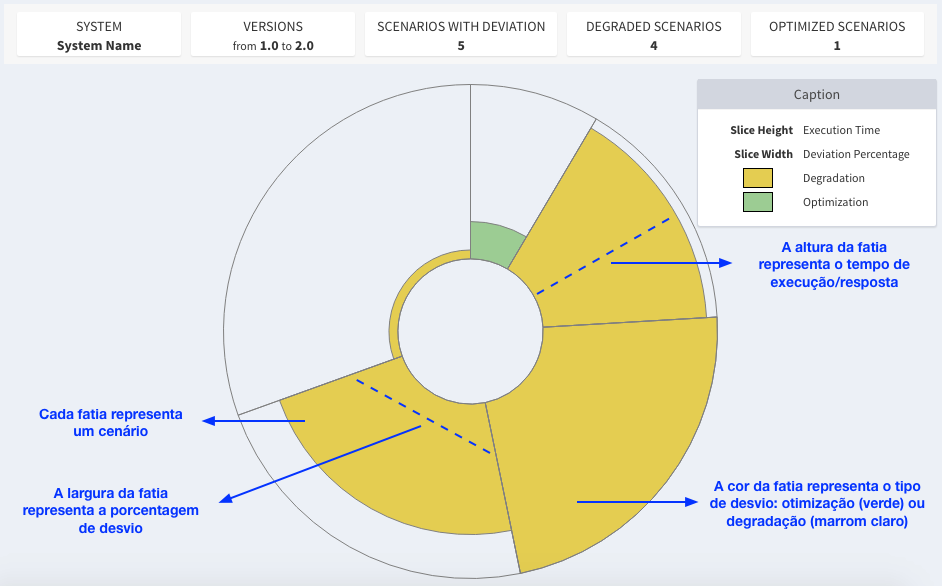
\includegraphics[scale=0.42]{Imagens/scenario_summarization_explicative_portuguese.png}

	\noindent \textit{\textbf{Questão 12.} Considerando a visualização "Sumarização de Cenários" da ferramenta acessada através do link {\(<\)}link\_para\_a\_ferramenta{\(>\)}, você consegue identificar qual cenário (isto é, caso de teste) possui maior desvio de desempenho (degradação ou melhoria do tempo de execução/tempo de resposta) dentre os exibidos? O cenário foi otimizado ou degradado?}
	\par
	\noindent \textit{\textbf{Questão 13.} Quão fácil foi responder à pergunta anterior?}
	\par
	\noindent \textit{\textbf{Questão 14.} Considerando a visualização "Sumarização de Cenários" da ferramenta acessada através do link {\(<\)}link\_para\_a\_ferramenta{\(>\)}, você consegue identificar qual cenário possui maior tempo de execução/resposta dentre os exibidos? O cenário foi otimizado ou degradado?}
	\par
	\noindent \textit{\textbf{Questão 15.} Quão fácil foi responder à pergunta anterior?}
	\par
	\noindent \textit{\textbf{Questão 16.} Você poderia mencionar aspectos dessa visualização que você gostou? E quais outros aspectos você não gostou? Você tem alguma sugestão de melhoria ou comentário para essa visualização?}
\end{framed}

\begin{framed}
	\noindent \textit{\textbf{Página 5/5 - Geral}}
	\par
	\noindent \textit{\textbf{Questão 17.} Você vê benefícios de usar a ferramenta de visualização de desvios de desempenho apresentada? Se sim, quais?}
	\par
	\noindent \textit{\textbf{Questão 18.} Você utilizaria a ferramenta como parte integrante do processo de desenvolvimento de software do \underline{Jetty/VRaptor}? Se sim, como você vislumbra que ela seria utilizada?}
	\par
	\noindent \textit{\textbf{Questão 19.} Utilize o espaço abaixo para incluir comentários adicionais que deseje.}
	\par
	\noindent \textit{\textbf{Questão 20.} Você está disponível para ser contactado para discutir nossos resultados relacionados ao projeto \underline{Jetty/VRaptor}? Se sim, por favor deixe o seu email abaixo.}

	\noindent \textit{Você pode acessar e verificar todos os resultados gerados pela nossa ferramenta através deste link: http://apvis.herokuapp.com/}
\end{framed}